\documentclass[letterpaper,journal]{IEEEtran}
\usepackage{amsmath,amsfonts}
\usepackage{algorithmic}
\usepackage{algorithm}
\usepackage{array}
\usepackage[caption=false,font=normalsize,labelfont=sf,textfont=sf]{subfig}
\usepackage{textcomp}
\usepackage{stfloats}
\usepackage{url}
\usepackage{verbatim}
\usepackage{graphicx}
\usepackage{cite}
\usepackage{tabularx}
\usepackage{booktabs}
\hyphenation{op-tical net-works semi-conduc-tor IEEE-Xplore}
% updated with editorial comments 8/9/2021

\begin{document}

\title{Optical Integrated Sensing and Communication for 6G: A Cross-Modality Survey and Metric-Governed Roadmap}

\author{Fatih D\"onmez, Ahmet Altuncu, and Mustafa Namdar,~\IEEEmembership{Member, IEEE}%
    \thanks{Fatih D\"onmez and Ahmet Altuncu are with the Department of Electrical and Electronics Engineering, Afyon Kocatepe University, Afyonkarahisar, Turkiye (e-mail: fatih.donmez@usr.aku.edu.tr; aaltuncu@aku.edu.tr). Fatih D\"onmez ORCID: 0000-0003-0553-4418. Corresponding author: Fatih D\"onmez.}%
    \thanks{Mustafa Namdar is with the Department of Electrical and Electronics Engineering, Faculty of Engineering, Kutahya Dumlupinar University, Kutahya, Turkiye (e-mail: mustafa.namdar@dpu.edu.tr).}}

\markboth{Draft Manuscript}%
{D\"onmez \MakeLowercase{\textit{et al.}}: Optical Integrated Sensing and Communication Review}

\maketitle

\begin{abstract}
    Optical Integrated Sensing and Communication (O-ISAC) is emerging as a 6G design direction because optical carriers can support high-rate links and sensing functions across guided fiber, free-space optical, VLC/LiFi, and photonics-assisted high-frequency platforms. Yet the literature remains fragmented by modality, terminology, measurement plane, and metric semantics, making direct comparison risky without an explicit governance layer.

    This systematic review synthesizes 220 peer-reviewed O-ISAC studies using a PRISMA-grounded process and develops a cross-modality taxonomy spanning medium class, integration mechanism, detection/observability regime, and sensing task. We introduce a metric-governed reporting contract that separates bandwidth-limited range resolution $\Delta r_{\min}$, estimator-level accuracy such as $\sigma_r$/RMSE, CRB/FIM bound statements, fiber spatial granularity $\Delta z$, and optical/electrical signal-quality planes. This contract enables conservative rate--resolution analysis and capacity-resolution quotient (CRQ) synthesis only when rate and sensing metrics are reported under compatible scenario records.

    The review further maps enabling technologies, including optical RIS/ORIS, optical phased arrays, photonic integration, photonics-assisted mmWave/THz generation, and ML/security-aware adaptation, and links them to deployment constraints and benchmark needs. The resulting roadmap identifies the reporting practice, taxonomy alignment, reproducible evaluation workflows, scalable hardware, and domain-aware validation needed for credible O-ISAC progress.
\end{abstract}

\begin{IEEEkeywords}
    Optical integrated sensing and communication, O-ISAC, free-space optics, visible light communication, distributed fiber sensing, photonic-terahertz systems, systematic review.
\end{IEEEkeywords}


\section{Introduction}
\label{introduction}

Integrated sensing and communication (ISAC) is now a core 6G design direction because future systems must exchange data and observe physical context in the same workflow \cite{O_ISAC_070,O_ISAC_162}. Optical integrated sensing and communication (O-ISAC) extends that premise onto optical carriers and therefore changes both the opportunity and the comparison problem. Fiber links, free-space optical links, VLC/LiFi systems, and photonics-assisted mmWave/THz chains do not share one channel model, receiver plane, or sensing metric vocabulary, even when they all use an O-ISAC label \cite{O_ISAC_021,O_ISAC_068,O_ISAC_303}. Fig.~\ref{fig:fig1} is retained as the opening landscape view because it captures the main physical motivation and modality split.

\begin{figure*}[!t]
    \centering
    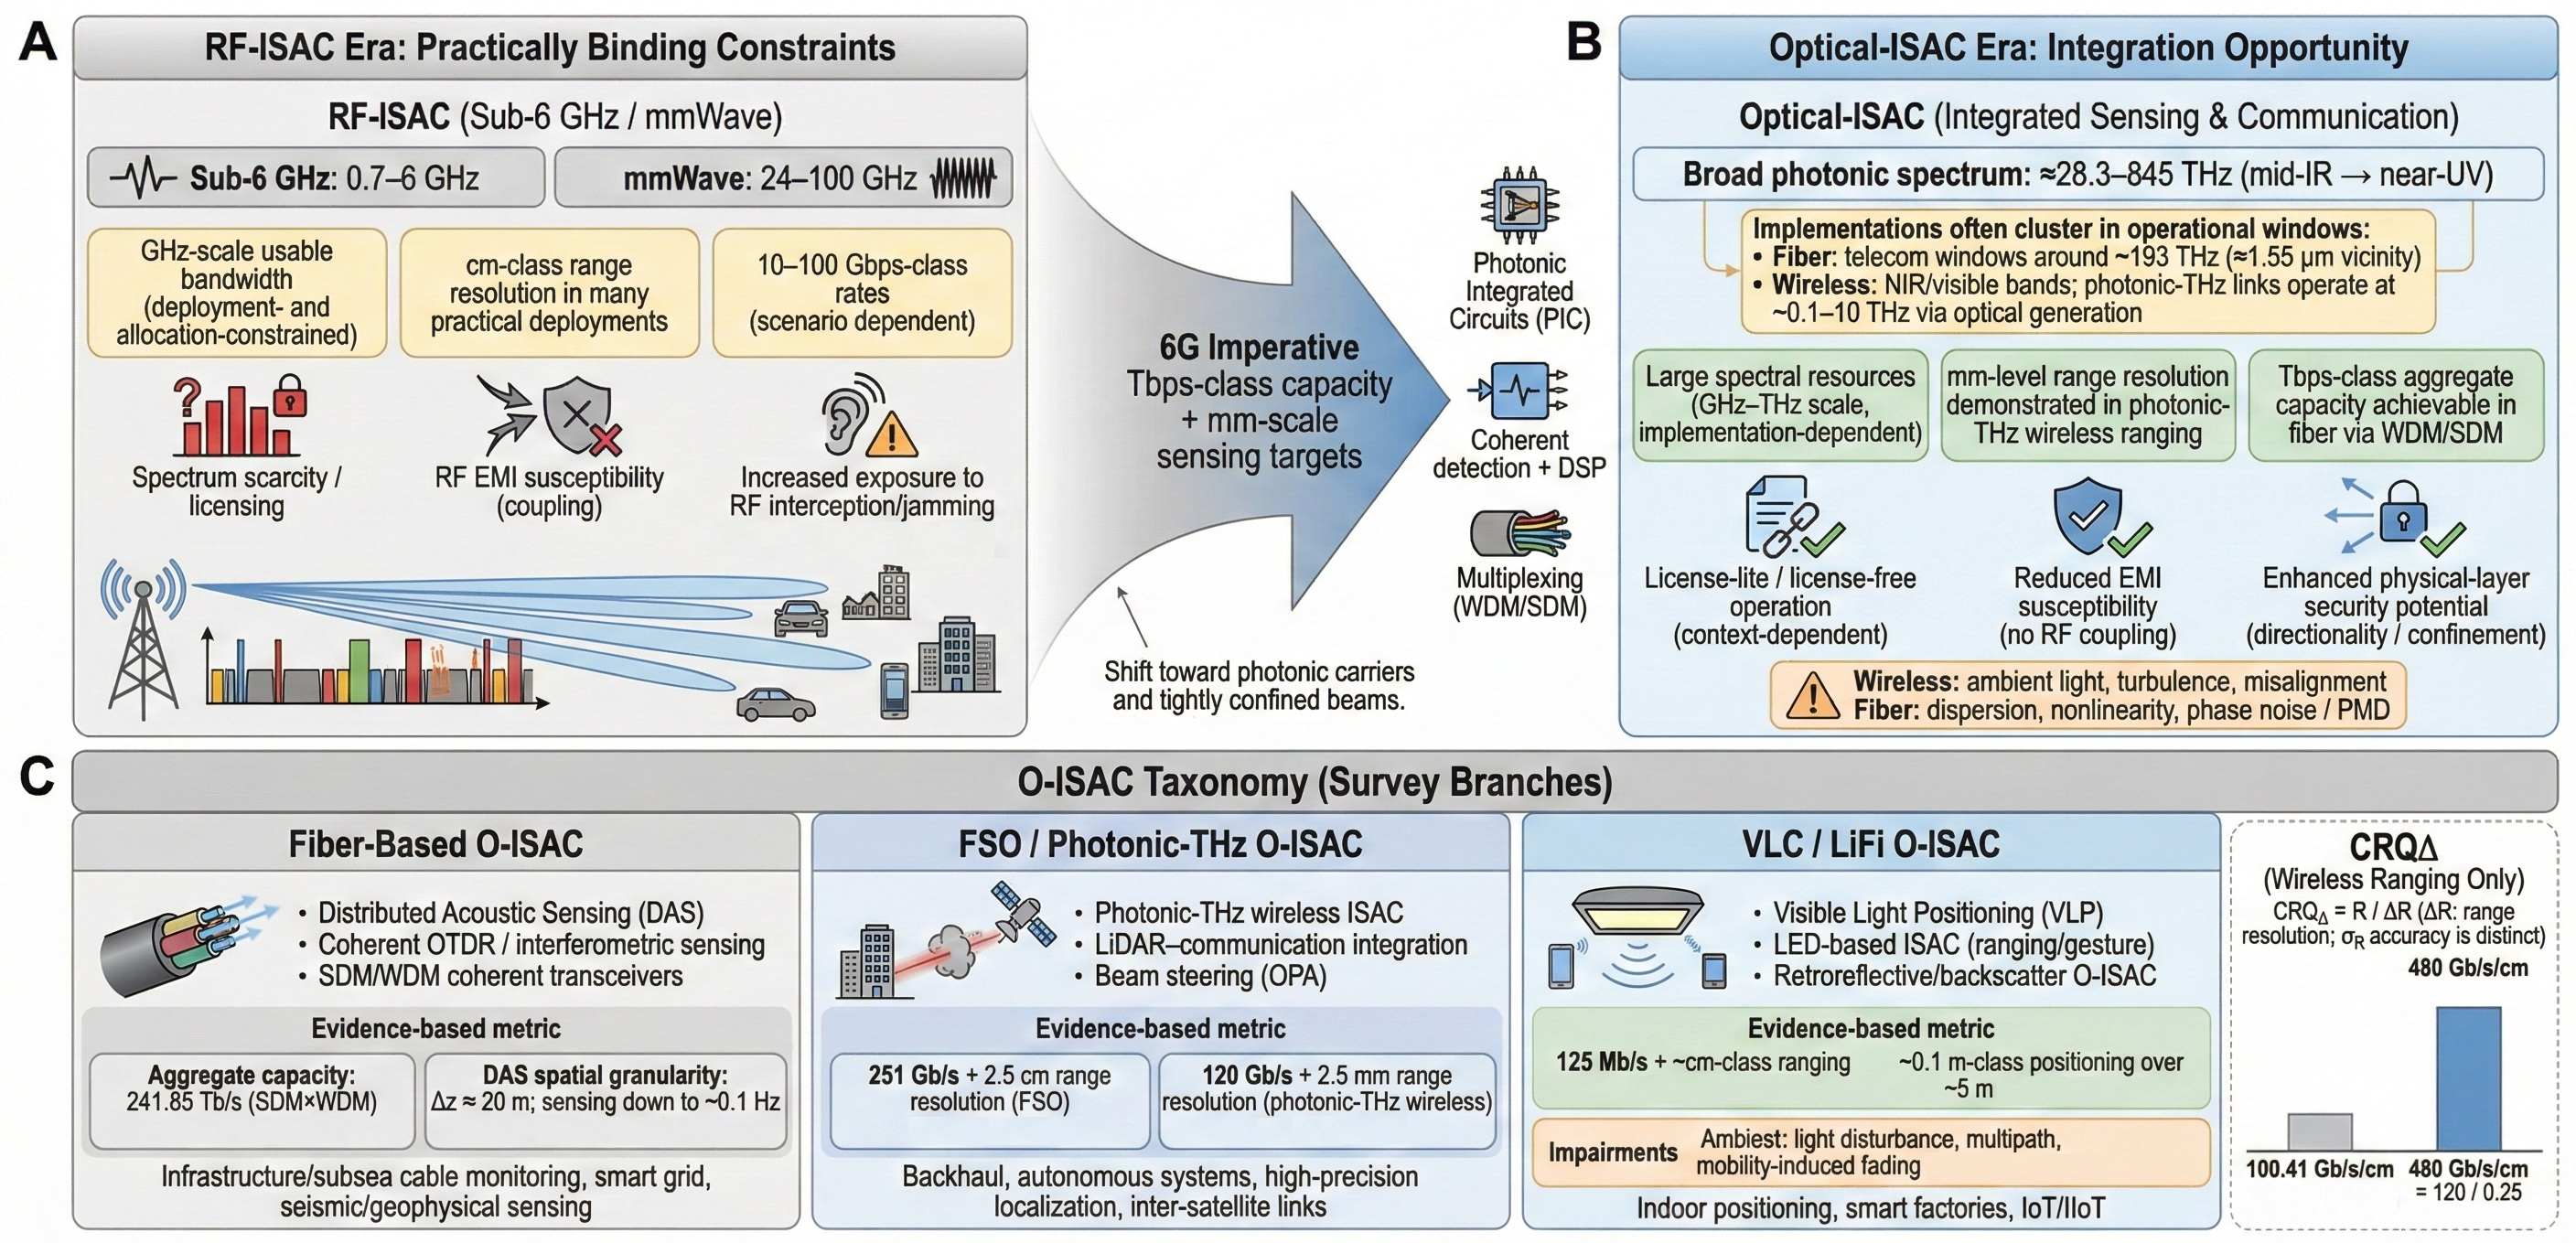
\includegraphics[width=\linewidth]{figures/fig1.jpg}
    \caption{O-ISAC landscape across optical spectrum resources and the main fiber, FSO/photonic-THz, and VLC/LiFi branches.}
    \label{fig:fig1}
\end{figure*}

The practical appeal is clear: photonic-THz demonstrations report wireless rates around 120 Gbps with millimeter-level range resolution, while multicore fiber experiments report aggregate transmission above 200 Tb/s with concurrent sensing \cite{O_ISAC_105,O_ISAC_046}. These results should not be pooled as if they were the same architecture. RF/mmWave ISAC remains constrained by spectrum scarcity, bandwidth-limited sensing, and high-frequency hardware complexity; optical systems open wider spectral resources but split into guided and wireless operating regimes with different impairments, calibration needs, and signal-quality reference planes \cite{O_ISAC_021,O_ISAC_203,O_ISAC_286}. The review therefore uses metric-governed comparison rather than headline performance ranking. Frequently used notation and acronyms are provided in the supplementary material.

\begin{table*}[!t]
    \caption{Related survey landscape and the contribution of this review.}
    \label{tab:axis_comparison}
    \centering
    \scriptsize
    \setlength{\tabcolsep}{2.4pt}
    \renewcommand{\arraystretch}{1.08}
    \begin{tabularx}{\textwidth}{@{}p{1.25cm}p{0.58cm}p{1.55cm}Xc c c c c@{}}
        \toprule
        Work & Year & Scope & Main emphasis & Syst. & Cross-med. & Tax. & Metric gov. & CRQ \\
        \midrule
        \cite{O_ISAC_161} & 2025 & RF/6G ISAC & RF-centric survey framing and standardization context & No & No & Part & No & No \\
        \cite{O_ISAC_068} & 2024 & VLC & Visible-light JCS prospects and indoor positioning links & No & No & Part & No & No \\
        \cite{O_ISAC_327} & 2024 & VLC/VLP & VLC/VLP channel and localization survey & No & No & Part & No & No \\
        \cite{O_ISAC_006} & 2024 & Fiber & Fiber-sensing ISAC challenges & No & No & Part & No & No \\
        \cite{O_ISAC_021} & 2024 & Optical ISAC & Architecture, potential, and challenge tutorial & No & Part & Part & Part & No \\
        \cite{O_ISAC_070} & 2026 & Photonic THz & Photonic THz-ISAC waveform/system view & No & Part & Part & No & Part \\
        \cite{O_ISAC_163} & 2025 & RIS/ISAC & RIS-enabled ISAC enabler context & No & No & Part & Part & No \\
        This review & 2026 & All optical & PRISMA $N=220$, taxonomy, metric contract, governed tradeoff, enablers, applications, roadmap & Yes & Yes & Yes & Yes & Yes \\
        \bottomrule
    \end{tabularx}
\end{table*}

The fragmentation challenge reduces to four fault lines: terminology aliasing across RadCom/JRC/VLC/photonic/fiber labels; metric non-isomorphism between $\Delta r_{\min}$, RMSE/$\sigma_r$, CRB/FIM, $\Delta z$, OSNR, and electrical SNR; modality siloing across fiber, FSO, VLC/LiFi, and photonic-THz communities; and weak cross-domain transfer of waveforms, calibration practice, and benchmarks. This review addresses those faults through five contributions: a PRISMA/TQAF evidence base, a cross-modality taxonomy, a metric-governed reporting contract, a governed rate--resolution and CRQ synthesis, and a compact deployment/enabler/roadmap map. The original RF--O-ISAC comparison table and introductory modality preview figure have been moved to the supplementary file for traceability.

\section{Background and Metric-Governance Contract}
\label{sec:background_metric_contract}

An O-ISAC system couples an optical source, modulation and waveform resources, a propagation medium, receiver observables, and communication/sensing estimators. The shared abstraction in Fig.~\ref{fig:fig_ii_1} is useful only if the modality-specific pieces remain visible: coherent receivers preserve complex-field information, IM/DD receivers expose intensity-domain observations, fiber channels are guided and dispersive/nonlinear, and wireless optical channels add geometry, turbulence, pointing, and ambient-light constraints \cite{O_ISAC_023,O_ISAC_039,O_ISAC_046,O_ISAC_056}. The conceptual NLSE and extended channel derivations are moved to the supplementary file; in the main text, their role is to remind the reader that guided propagation, wireless propagation, and photonic high-frequency generation are not interchangeable channel assumptions.

\begin{figure*}[!t]
    \centering
    
\includegraphics[width=\linewidth]{figures/fig_ii_1.png}
    \caption{Unified O-ISAC source--channel--observation abstraction with modality-specific propagation and receiver planes retained.}
    \label{fig:fig_ii_1}
\end{figure*}

\begin{table*}[!t]
    \caption{Modality-aware O-ISAC abstraction.}
    \label{tab:ii1}
    \centering
    \scriptsize
    \setlength{\tabcolsep}{2.7pt}
    \renewcommand{\arraystretch}{1.08}
    \begin{tabularx}{\textwidth}{@{}p{1.65cm}p{2.05cm}p{2.15cm}p{2.0cm}X@{}}
        \toprule
        Modality & Channel basis & Receiver/observable & Typical task & Governance warning \\
        \midrule
        Fiber & Guided dispersive/nonlinear link; DAS/DFOS granularity & Coherent or direct optical/electrical plane & Vibration, strain, intrusion, co-route monitoring & Report $\Delta z$ and OSNR plane; do not call it wireless range resolution \\
        FSO & LoS optical wireless with turbulence and pointing & Direct or coherent photodetection & Ranging, tracking, link adaptation & Geometry and weather condition admissibility dominate comparison \\
        VLC/LiFi & Lambertian LoS/NLoS indoor optical wireless & Mostly IM/DD, sometimes camera-assisted & Localization, gesture, indoor sensing & Electrical SNR/RMSE cannot be merged with optical OSNR or CRB without model disclosure \\
        Photonic-THz/hybrid & Optical generation/distribution plus mmWave/THz or mixed links & Coherent photonic, electronic, or hybrid chains & High-rate ranging and fiber-wireless transfer & Separate optical generation, wireless propagation, and post-detection measurement planes \\
        \bottomrule
    \end{tabularx}
\end{table*}

The protected metric contract is summarized in Table~\ref{tab:ii2}. Bandwidth-limited range resolution is
\begin{equation}
    \Delta r_{\min}=\frac{v}{2B_{\mathrm{eff}}},
    \label{eq:range_resolution}
\end{equation}
with $v=c$ in free space and $v\approx c/n_g$ in guided media when a two-way convention is appropriate. It is not estimator accuracy. Accuracy terms such as RMSE and $\sigma_r$ depend on SNR, geometry, estimator choice, and data model. CRB/FIM statements are bound-level claims under explicit observation assumptions. Fiber spatial granularity $\Delta z$ is a gauge/segment property rather than a free-space range-resolution substitute. OSNR, post-detection electrical SNR, ESNR, and simulation SNR must remain plane-tagged.

\begin{table*}[!t]
    \caption{Metric contract for admissible O-ISAC comparison.}
    \label{tab:ii2}
    \centering
    \scriptsize
    \setlength{\tabcolsep}{2.8pt}
    \renewcommand{\arraystretch}{1.08}
    \begin{tabularx}{\textwidth}{@{}p{2.15cm}p{2.15cm}p{2.7cm}X@{}}
        \toprule
        Metric object & Valid role & Must report & Forbidden shortcut \\
        \midrule
        $\Delta r_{\min}$ & Bandwidth-limited resolution & $B_{\mathrm{eff}}$, propagation convention, scenario & Replacing RMSE or CRB with resolution \\
        $\sigma_r$/RMSE & Estimator-level accuracy & estimator, SNR plane, geometry, dataset/simulation setup & Treating as bandwidth-only resolution \\
        CRB/FIM & Bound context & observation model, parameters, noise statistics & Treating as measured accuracy \\
        $\Delta z$ & Fiber spatial granularity & gauge length/segment, interrogator assumptions & Treating as wireless range resolution \\
        OSNR/SNR/ESNR & Signal-quality plane & optical/electrical/reference location and bandwidth & Mixing planes without receiver/noise model \\
        $\mathrm{CRQ}_{\Delta}$ & Rate per bandwidth-limited resolution & matched $R$ and $\Delta r_{\min}$ in one scenario record & Combining unmatched rate and sensing entries \\
        \bottomrule
    \end{tabularx}
\end{table*}

For the governed synthesis, the capacity-resolution quotient is used only as
\begin{equation}
    \mathrm{CRQ}_{\Delta}=\frac{R}{\Delta r_{\min}},
    \label{eq:crq_delta}
\end{equation}
and only when the rate and $\Delta r_{\min}$ belong to the same scenario record. The broader optimization view is therefore reduced here to a bridge: Section~\ref{sec:tradeoff} interprets performance clouds only after the taxonomy axes and metric roles have been aligned.

\section{Review Methodology}
\label{sec:methodology}

This review follows PRISMA 2020 and PRISMA-S search-reporting principles. The protocol was registered with OSF on February 12, 2026 (Registration ID: \texttt{7f6wb}), and the formal database search used IEEE Xplore, Scopus, and Web of Science, frozen on November 30, 2025. Exact search strings, search-stage audit material, and moved method-detail tables are preserved in the supplementary evidence package rather than repeated in the main manuscript.

\begin{table*}[!t]
    \caption{Compact eligibility criteria used for study selection.}
    \label{tab:iii1}
    \centering
    \scriptsize
    \setlength{\tabcolsep}{3pt}
    \renewcommand{\arraystretch}{1.08}
    \begin{tabularx}{\textwidth}{@{}p{2.4cm}X X@{}}
        \toprule
        Criterion & Include & Exclude \\
        \midrule
        Topical scope & Optical, fiber, FSO, VLC/LiFi, photonic-mmWave/THz, or hybrid systems with both sensing and communication relevance & Pure communication, pure sensing, or non-optical RF-only ISAC without optical relevance \\
        Evidence type & Peer-reviewed articles, conference papers, and survey/review works needed for context & Editorial-only, incomplete metadata, inaccessible, or duplicate records outside the audit ledger \\
        Synthesis value & Reports architecture, metric, modality, experiment/simulation, or application information usable for taxonomy/TQAF extraction & No usable O-ISAC extraction fields after full-text assessment \\
        \bottomrule
    \end{tabularx}
\end{table*}

\begin{figure}[!t]
    \centering
    \fbox{\begin{minipage}{0.92\linewidth}
        \centering
        \footnotesize
        IEEE Xplore + Scopus + Web of Science search frozen on Nov. 30, 2025\\[2pt]
        $\downarrow$ deduplication and title/abstract screening\\[2pt]
        222 full texts assessed\\[2pt]
        $\downarrow$ 2 full-text exclusions\\[2pt]
        Final PRISMA corpus: $N=220$ peer-reviewed studies
    \end{minipage}}
    \caption{Compressed PRISMA flow for the final O-ISAC corpus.}
    \label{fig:fig_iii_1}
\end{figure}

The TQAF appraisal used five compact dimensions: topical fit, metric transparency, modality/implementation clarity, methodological reproducibility, and contribution relevance to cross-modality synthesis. Data extraction recorded medium, integration, detection/observability, sensing task, communication metrics, sensing metrics, signal-quality plane, and scenario compatibility. The final corpus includes 222 full texts assessed, 2 full-text exclusions, and $N=220$ included studies. The bibliography remains aligned with the included-corpus ledger; a small audit-tail is retained for traceability rather than treated as primary evidence in the narrative.

\section{Unified O-ISAC Taxonomy}
\label{sec:taxonomy}

The taxonomy keeps ambiguity visible instead of forcing all papers into a single optical-ISAC mold. Each paper $p$ is mapped as
\begin{equation}
    T(p)=\bigl(m(p),i(p),d(p),s(p)\bigr),
    \label{eq:taxonomy_vector}
\end{equation}
where $m$ is medium class, $i$ is integration class, $d$ is detection/observability class, and $s$ is sensing task. The detailed operational contract and the former medium/integration/detection cluster tables are moved to the supplementary file; Table~\ref{tab:taxonomy_compact} keeps the main-text synthesis. Counts indicate evidence concentration, not technical superiority.

\begin{figure*}[!t]
    \centering
    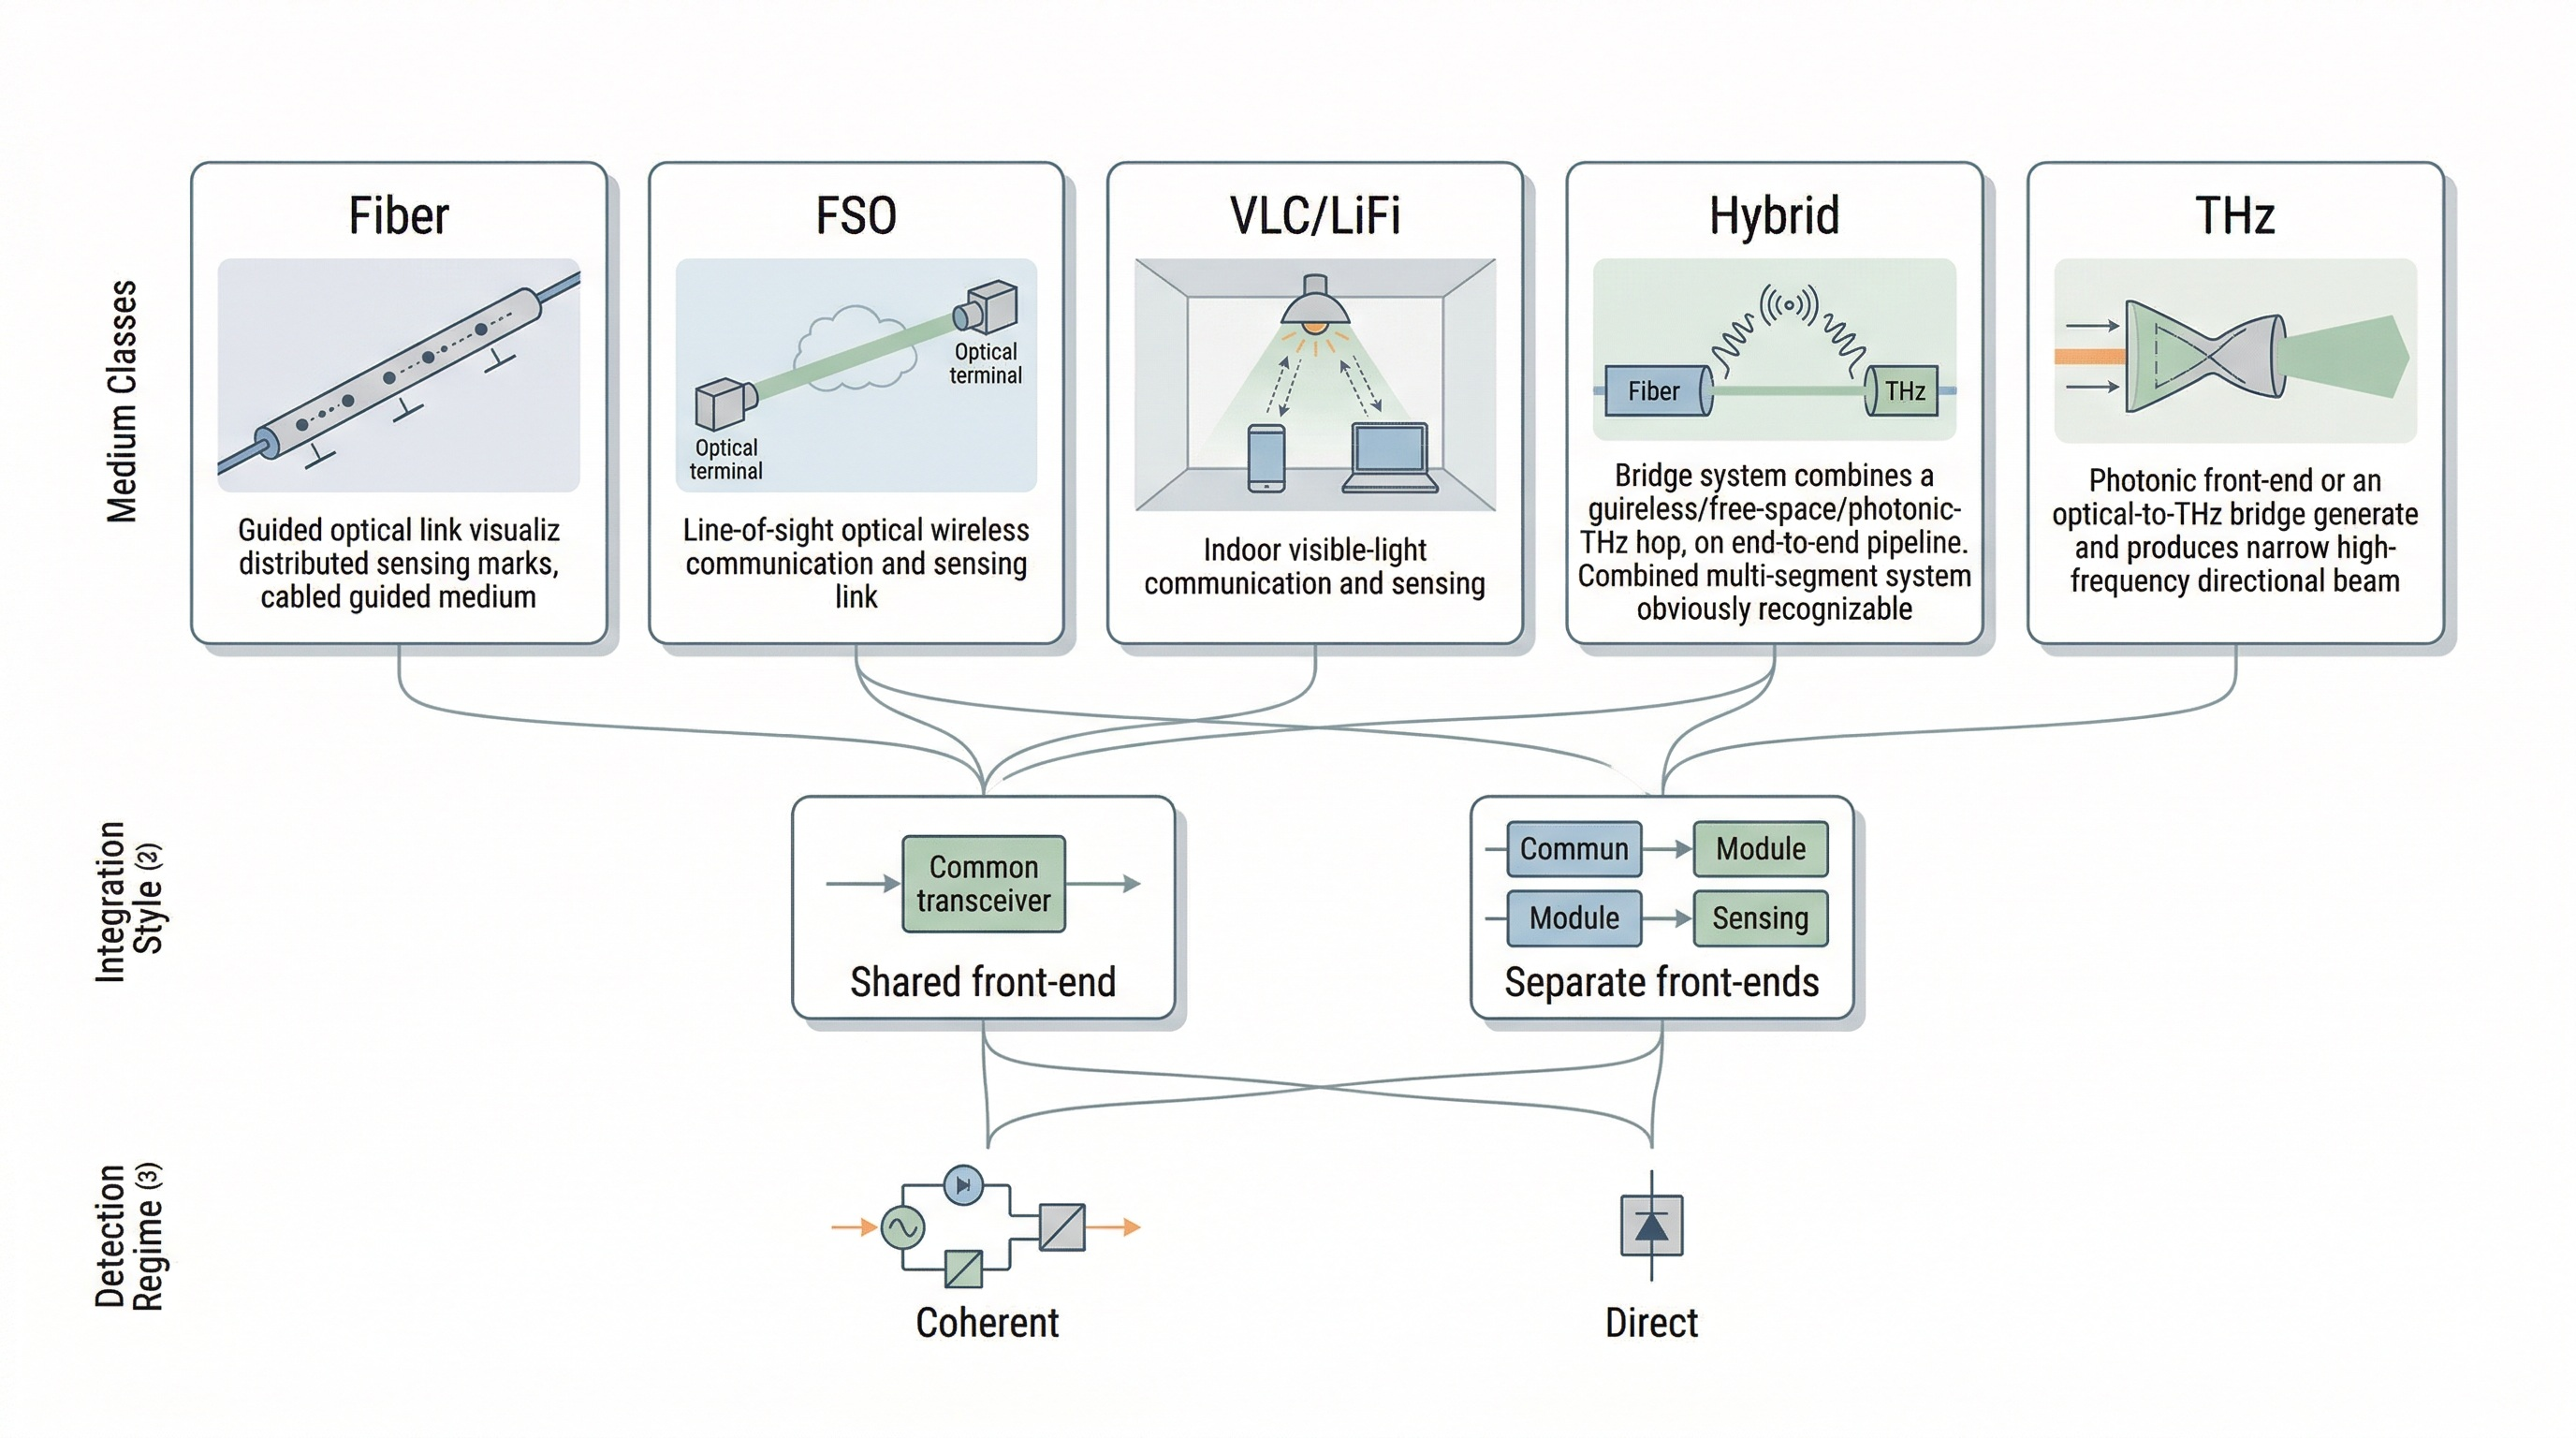
\includegraphics[width=\linewidth,trim=0.8cm 0.7cm 0.8cm 1.1cm,clip]{figures/fig_iv_1.jpg}
    \caption{Semantic taxonomy map retained as the single main-text taxonomy figure.}
    \label{fig:fig_iv_1}
\end{figure*}

\begin{table*}[!t]
    \caption{Compact taxonomy summary across the $N=220$ corpus.}
    \label{tab:taxonomy_compact}
    \centering
    \scriptsize
    \setlength{\tabcolsep}{2.7pt}
    \renewcommand{\arraystretch}{1.08}
    \begin{tabularx}{\textwidth}{@{}p{2.0cm}p{1.65cm}p{2.25cm}p{2.2cm}X@{}}
        \toprule
        Medium & Corpus share & Dominant detection & Dominant task & Governance warning \\
        \midrule
        Fiber & 45/220 & Coherent-leading, with direct tail & Range/vib. monitoring & Compare using guided-channel and $\Delta z$/OSNR semantics \\
        FSO & 19/220 & Mixed direct/coherent & Ranging-heavy & Condition on geometry, turbulence, and pointing assumptions \\
        VLC/LiFi & 25/220 & Direct IM/DD & Localization and ranging & Electrical-plane accuracy dominates; do not infer optical OSNR behavior \\
        Photonic-THz / hybrid & 116/220 hybrid; 39 photonic-THz anchors & Near-balanced coherent/direct & Ranging-heavy with broad multi-task tail & Separate optical generation/distribution from wireless propagation and receiver plane \\
        \bottomrule
    \end{tabularx}
\end{table*}

Fiber O-ISAC is the guided anchor, with 45 records dominated by shared-front-end integration and a task mix spanning ranging, vibration, strain, and infrastructure monitoring \cite{O_ISAC_006,O_ISAC_041,O_ISAC_046}. FSO is smaller but strongly ranging-oriented, so its evidence should be read through weather, pointing, and geometry constraints \cite{O_ISAC_023,O_ISAC_035}. VLC/LiFi is the direct-detection and localization-oriented branch, where Lambertian channels and indoor deployment assumptions govern comparability \cite{O_ISAC_009,O_ISAC_039,O_ISAC_068}. Photonic-THz and hybrid systems form the broadest bridge class, linking optical generation/distribution, fiber-wireless transport, and high-frequency wireless sensing/communication \cite{O_ISAC_029,O_ISAC_070,O_ISAC_077,O_ISAC_105}. Across all four, taxonomy is a conditioning layer for Section~\ref{sec:tradeoff}, not a ranking table.

\section{Communication-Sensing Tradeoff Synthesis}
\label{sec:tradeoff}

The governed tradeoff synthesis is the core analytical result and is preserved. Across the $N=220$ paper corpus, the extraction produced 225 scenario points. Only 20 scenario records support rate plus $\Delta r_{\min}$, only 16 support rate plus $\sigma_r$/RMSE, and only 13 support the full rate--$\Delta r_{\min}$--$\sigma_r$ triplet. The sparse governed subset is therefore not a data-cleaning accident; it is evidence that O-ISAC reporting remains too heterogeneous for broad rate--sensing frontier claims.

\begin{table*}[!t]
    \caption{Governance attrition from reported metrics to admissible synthesis.}
    \label{tab:governance_attrition}
    \centering
    \scriptsize
    \setlength{\tabcolsep}{3pt}
    \renewcommand{\arraystretch}{1.08}
    \begin{tabularx}{\textwidth}{@{}p{2.8cm}p{2.0cm}p{2.2cm}X@{}}
        \toprule
        Evidence layer & Available count & Main retained use & Main attrition cause \\
        \midrule
        Scenario records & 225 & Corpus-level context & Heterogeneous reporting and modality planes \\
        Rate + $\Delta r_{\min}$ & 20 & CRQ-admissible resolution view & Missing matched bandwidth-limited resolution \\
        Rate + $\sigma_r$/RMSE & 16 & Accuracy-conditioned operating view & Missing estimator/SNR/geometry detail \\
        Full triplet & 13 & Most conservative cross-metric subset & Rate, resolution, and accuracy rarely co-reported \\
        \bottomrule
    \end{tabularx}
\end{table*}

\begin{figure*}[!t]
    \centering
    
\includegraphics[width=\linewidth]{figures/fig_v_1.png}
    \caption{Governed rate--resolution and rate--accuracy operating clouds after metric-role filtering.}
    \label{fig:fig_v_1}
\end{figure*}

\begin{table*}[!t]
    \caption{Governed fiber, wireless, and hybrid slices.}
    \label{tab:comparative_slices}
    \centering
    \scriptsize
    \setlength{\tabcolsep}{2.8pt}
    \renewcommand{\arraystretch}{1.08}
    \begin{tabularx}{\textwidth}{@{}p{1.7cm}p{2.0cm}p{2.1cm}X@{}}
        \toprule
        Slice & Strong evidence & Weakness for pooling & Main reading \\
        \midrule
        Fiber & Tb/s-class aggregate links and distributed sensing \cite{O_ISAC_046} & $\Delta z$ and OSNR differ from wireless range/ESNR & Guided infrastructure and monitoring anchor \\
        Wireless optical & FSO/VLC ranging/localization and OPA-controlled optical wireless links \cite{O_ISAC_023,O_ISAC_061} & Geometry, turbulence, ambient light, and estimator differences & Scenario-conditioned sensing/communication tradeoff \\
        Photonic-THz/hybrid & High-rate photonic generation plus mmWave/THz ranging \cite{O_ISAC_029,O_ISAC_105} & Optical and wireless planes can be conflated & Bridge class, not a single medium \\
        \bottomrule
    \end{tabularx}
\end{table*}

Fig.~\ref{fig:fig_v_1} is therefore the main governed operating-cloud figure. The former sparse CRQ frontier figure is moved to the supplementary file because its correct interpretation is narrow: it illustrates the two nondominated points inside the 20-point CRQ-valid subset, not a stable design envelope for the field. The main conclusion is stronger and safer in text: CRQ is useful only for matched rate and $\Delta r_{\min}$ scenario records, and current reporting practice leaves that subset sparse.

\section{Enabling Technologies and System-Level Co-Design}
\label{sec:enablers}

Enablers are retained as a compact synthesis because they explain how the taxonomy and metric contract may become deployable systems. Table~\ref{tab:vi_a_enablers} keeps one main-text enabler table; the broader enabler landscape figure and optimization scaffolding equations are moved to the supplementary file.

\begin{table*}[!t]
    \caption{Compact enabler synthesis for O-ISAC.}
    \label{tab:vi_a_enablers}
    \centering
    \scriptsize
    \setlength{\tabcolsep}{2.8pt}
    \renewcommand{\arraystretch}{1.08}
    \begin{tabularx}{\textwidth}{@{}p{2.15cm}p{2.65cm}p{2.3cm}X@{}}
        \toprule
        Enabler & Main O-ISAC role & Evidence center & Reporting risk \\
        \midrule
        ORIS / optical RIS & Programmable reflection, beam control, spatial reuse & Optical wireless and RIS-adjacent ISAC \cite{O_ISAC_163} & Geometry and control overhead must be disclosed \\
        OPA & Beam steering and joint communication/sensing aperture & OPA-based optical wireless ISAC \cite{O_ISAC_061,O_ISAC_091} & Beam pattern, scan schedule, and sensing estimator must be linked \\
        PIC / photonic integration & Compact source/modulator/receiver integration & Fiber-wireless and chip-scale demonstrations \cite{O_ISAC_036,O_ISAC_045} & Device results need system-level metric planes \\
        Photonics-assisted mmWave/THz & High-frequency generation/distribution and coherent reception & W-band, D-band, and THz-over-fiber systems \cite{O_ISAC_029,O_ISAC_070} & Separate optical generation from wireless propagation \\
        ML/security adaptation & Inference, calibration, robustness, and attack-aware control & Learning-assisted VLC/fiber-wireless studies \cite{O_ISAC_039,O_ISAC_242} & Dataset, generalization, and threat model must be explicit \\
        \bottomrule
    \end{tabularx}
\end{table*}

\begin{figure*}[!t]
    \centering
    
\includegraphics[width=\linewidth]{figures/fig_vi_2.jpg}
    \caption{Deployment-oriented systems map linking optical enablers, impairments, control, and benchmark discipline.}
    \label{fig:fig_vi_2}
\end{figure*}

\begin{table}[!t]
    \caption{Minimum reproducible reporting fields.}
    \label{tab:vi_d_reporting}
    \centering
    \scriptsize
    \setlength{\tabcolsep}{2.5pt}
    \renewcommand{\arraystretch}{1.05}
    \begin{tabularx}{\linewidth}{@{}p{1.8cm}X@{}}
        \toprule
        Field & Required disclosure \\
        \midrule
        Scenario & medium, geometry, range, mobility, weather/ambient state \\
        Link & rate, BER/throughput method, bandwidth, modulation, multiplexing \\
        Sensing & task, $\Delta r_{\min}$ or $\Delta z$, RMSE/$\sigma_r$, CRB/FIM if used \\
        Plane & OSNR/SNR/ESNR reference point and conversion model if any \\
        Evidence & simulation/experiment, data/code availability, uncertainty reporting \\
        \bottomrule
    \end{tabularx}
\end{table}

For this pass, multi-user resource optimization and secrecy/security optimization equations are no longer numbered in the main text. Their conceptual message remains: enablers become useful only when control variables, impairment models, and benchmark fields are reported together. AI/ML is treated as one adaptation layer rather than a standalone maturity claim.

\section{Applications and Use Cases Across Domains}
\label{sec:applications}

The application evidence is compressed to a deployment map rather than a maturity scorecard. Table~\ref{tab:section7_portfolio} replaces the longer portfolio and audit layer; the original application figure and dual-view consistency table are preserved in the supplementary file.

\begin{table*}[!t]
    \caption{Application portfolio compressed to five macro-domains.}
    \label{tab:section7_portfolio}
    \centering
    \scriptsize
    \setlength{\tabcolsep}{2.8pt}
    \renewcommand{\arraystretch}{1.08}
    \begin{tabularx}{\textwidth}{@{}p{2.35cm}p{2.6cm}p{2.55cm}X@{}}
        \toprule
        Macro-domain & Communication motif & Sensing motif & Transfer warning \\
        \midrule
        Smart infrastructure / cabled-fiber corridor & High-capacity transport and monitoring overlays & Vibration, strain, intrusion, seismic/corridor awareness & Strong for guided infrastructure; weak as wireless baseline \\
        Indoor VLC/LiFi localization & Lighting/data access and room-scale links & Positioning, gesture, occupancy, camera-assisted sensing & Direct-detection and ambient-light assumptions dominate \\
        Automotive / optical V2X & Short-range optical links and beam-controlled access & Ranging, pose, cooperative perception & Geometry, eye safety, weather, and blockage must be disclosed \\
        Underwater or harsh OWC & Optical wireless where RF is limited & Salinity, environmental, and link-state monitoring & Medium absorption/scattering makes transfer highly conditional \\
        LEO/satellite or space photonic O-ISAC & Space/NTN optical backhaul and hybrid network support & Tracking, ranging, situational awareness & Evidence is roadmap-oriented and needs deployment validation \\
        \bottomrule
    \end{tabularx}
\end{table*}

Across these domains, the recurring motif is not that one application is mature across all optical media. Instead, each domain inherits a specific observation plane and deployment constraint: fiber corridors inherit $\Delta z$ and OSNR semantics, indoor VLC/LiFi inherits IM/DD localization assumptions, vehicular optical links inherit geometry and blockage sensitivity, harsh OWC inherits medium-specific attenuation, and satellite/LEO cases inherit pointing and network-integration constraints \cite{O_ISAC_003,O_ISAC_005,O_ISAC_030,O_ISAC_059,O_ISAC_064}. The application map is therefore used to identify where methods may transfer and where the taxonomy should block unsafe analogy.

\section{Open Challenges and Research Roadmap}
\label{sec:roadmap}

The roadmap is compressed to one figure, one challenge table, and one five-row agenda. Fig.~\ref{fig:fig_viii_1} remains the main roadmap graphic because it links the challenge domains back to metric governance, enablers, and applications.

\begin{figure*}[!t]
    \centering
    
\includegraphics[width=\linewidth]{figures/fig_viii_1.jpg}
    \caption{Challenge-to-roadmap dependency map for taxonomy, metrics, benchmarks, hardware, security, and deployment validation.}
    \label{fig:fig_viii_1}
\end{figure*}

\begin{table*}[!t]
    \caption{Compressed O-ISAC challenge domains.}
    \label{tab:challenge_compact}
    \centering
    \scriptsize
    \setlength{\tabcolsep}{2.8pt}
    \renewcommand{\arraystretch}{1.08}
    \begin{tabularx}{\textwidth}{@{}p{2.4cm}p{3.0cm}X@{}}
        \toprule
        Domain & Bottleneck & Roadmap response \\
        \midrule
        Std./interoperability & Terminology, taxonomy, and reporting fields remain inconsistent & Shared O-ISAC taxonomy, PRISMA-style ledgers, metric-governed templates \\
        Hardware scalability & OPA/ORIS/PIC/photonic-THz demonstrations are promising but unevenly integrated & Co-design aperture, source, receiver, calibration, and packaging metrics \\
        Channel modeling/evaluation & Fiber, FSO, VLC, and photonic-THz assumptions are often mixed & Scenario-tagged benchmark channels and plane-aware signal-quality reporting \\
        Security/reliability & ML, sensing data, and narrow-beam control add new attack and failure surfaces & Threat-modeled evaluation with robustness and privacy fields \\
        Deployment convergence & Application claims outpace cross-domain validation & Domain-aware pilots tied to reproducible evaluation workflows \\
        \bottomrule
    \end{tabularx}
\end{table*}

\begin{table*}[!t]
    \caption{Five-item prioritized research agenda.}
    \label{tab:viii_f_2}
    \centering
    \scriptsize
    \setlength{\tabcolsep}{2.8pt}
    \renewcommand{\arraystretch}{1.08}
    \begin{tabularx}{\textwidth}{@{}p{0.55cm}p{2.7cm}X p{2.15cm}@{}}
        \toprule
        Pri. & Agenda item & Concrete deliverable & Risk if deferred \\
        \midrule
        1 & Metric-governed reporting & Required fields for rate, $\Delta r_{\min}$, $\sigma_r$/RMSE, CRB/FIM, $\Delta z$, OSNR/SNR plane & Persistent unsafe comparisons \\
        2 & Reproducible corpus workflow & Public ledgers, search strings, extraction sheets, and code for figures/tables & Weak systematic-review traceability \\
        3 & Cross-modality benchmarks & Fiber/FSO/VLC/photonic-THz scenario templates with uncertainty reporting & Non-transferable performance claims \\
        4 & Scalable hardware evidence & OPA/ORIS/PIC/photonic-THz prototypes evaluated with shared fields & Enabler claims remain isolated \\
        5 & Deployment validation & Domain pilots for infrastructure, indoor, vehicle, harsh OWC, and space/NTN cases & Application map remains aspirational \\
        \bottomrule
    \end{tabularx}
\end{table*}

The removed roadmap utility and governance equations were organizational scaffolding, not necessary technical contributions. The remaining roadmap message is direct: O-ISAC needs interoperable taxonomy, metric-governed reporting, reproducible benchmarks, scalable hardware, and deployment validation.

\section{Conclusions}
\label{sec:conclusion}

This review synthesized optical integrated sensing and communication as a family of architectures rather than a monolithic interchangeable design space. Using a PRISMA-grounded corpus of 220 studies, it organized fiber, FSO, VLC/LiFi, photonic-THz, and hybrid work through a cross-modality taxonomy and a metric-governed comparison contract. The central lesson is that comparability requires explicit modality, metric role, measurement plane, and deployment context: $\Delta r_{\min}$ is not $\sigma_r$/RMSE, CRB/FIM is a bound-level statement, fiber $\Delta z$ is not wireless range resolution, and OSNR and electrical SNR cannot be exchanged without a receiver/noise model. Under that governed reading, the rate--resolution evidence is informative but sparse: only small subsets of the 225 extracted scenario records support admissible CRQ or full triplet synthesis. Future progress therefore depends as much on reporting practice as on hardware advances. Reproducible workflows, benchmark definitions, scalable OPA/ORIS/PIC and photonic-THz hardware, security-aware adaptation, and domain-aware validation are the necessary path from promising O-ISAC demonstrations to credible 6G systems.

\nocite{*}

\bibliographystyle{IEEEtran}
\bibliography{IEEEabrv, references} % referanslarim.bib dosyanın adını buraya yazmalısın





\newpage

\begin{IEEEbiography}[{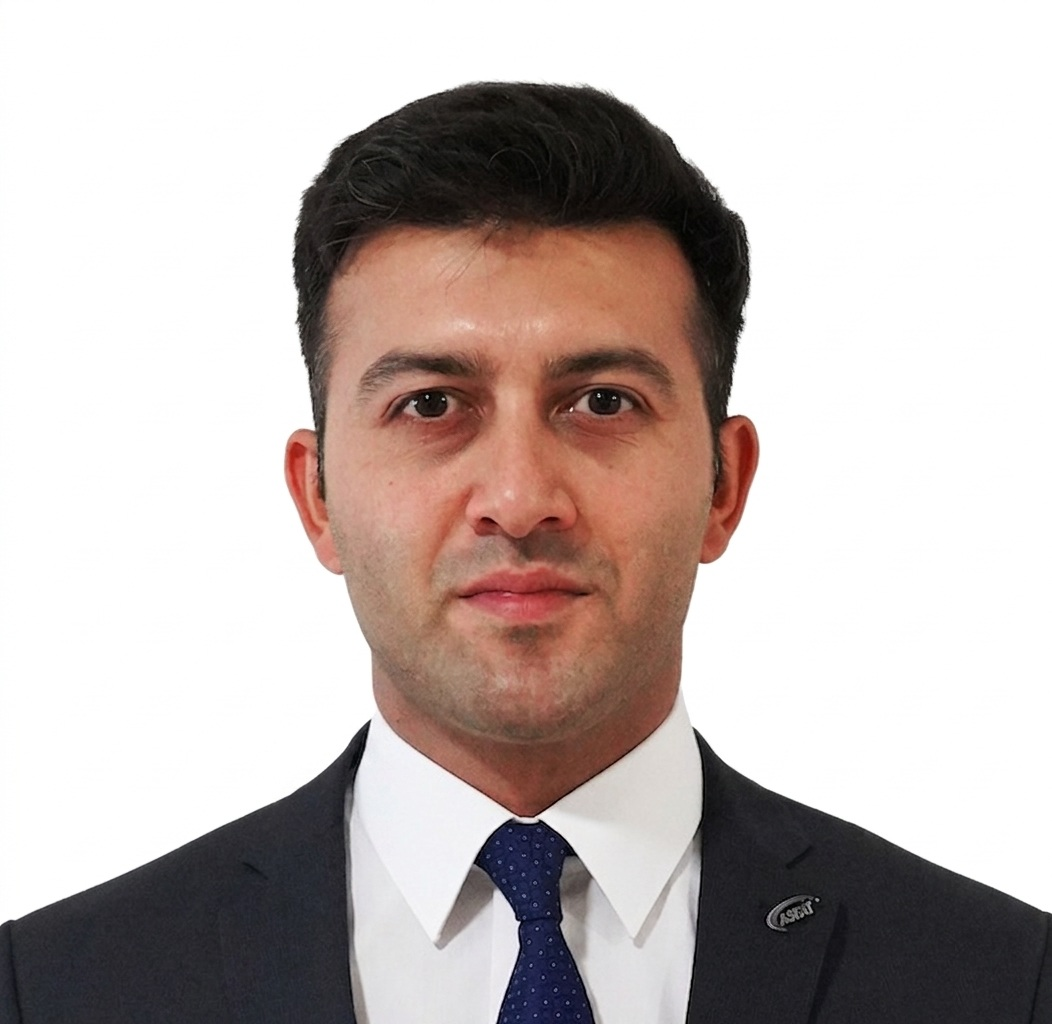
\includegraphics[width=1in,height=1.25in,clip,keepaspectratio]{figures/foto_fatih.jpg}}]{Fatih D\"onmez}
    received the B.S. degree in electrical and electronics engineering from TOBB University of Economics and Technology, Ankara, Turkiye, in 2012, and the M.S. degree in electrical and electronics engineering from Kutahya Dumlupinar University, Kutahya, Turkiye, in 2022. He is currently pursuing the Ph.D. degree in electrical and electronics engineering with Afyon Kocatepe University, Afyonkarahisar, Turkiye. His research interests include communication networks, wireless communications, communication system optimization, and integrated sensing and communication (ISAC).
\end{IEEEbiography}

\begin{IEEEbiography}[{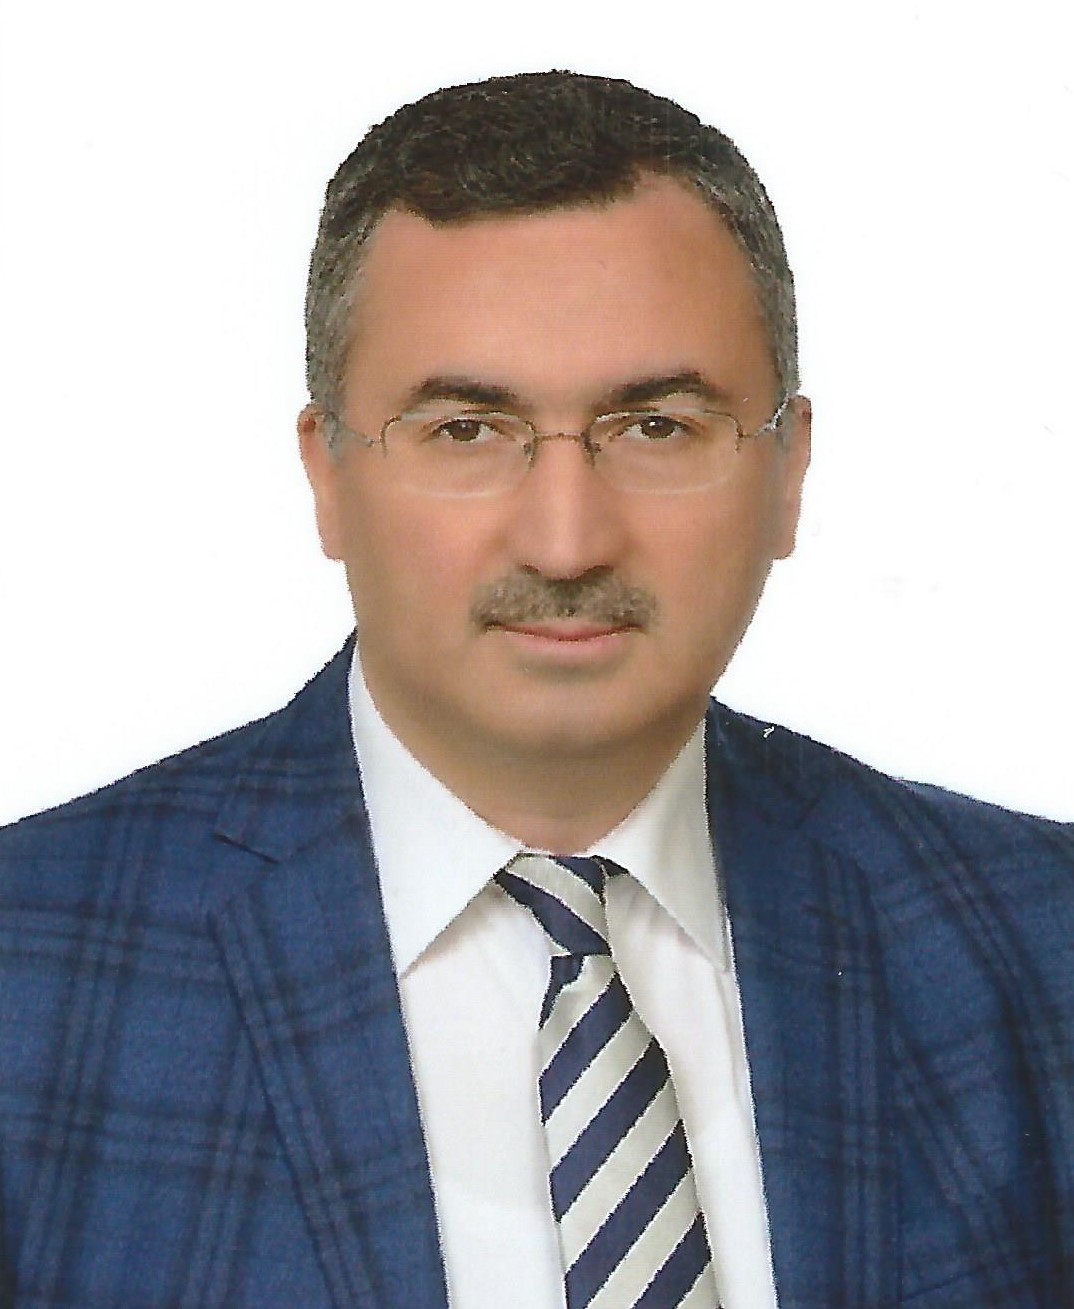
\includegraphics[width=1in,height=1.25in,clip,keepaspectratio]{figures/foto_ahmet.jpg}}]{Ahmet Altuncu}
    received the Ph.D. degree in electronic systems engineering from the University of Essex, Colchester, U.K., in 1998. He founded and directed the Photonics Technologies Application and Research Center at Dumlupinar University. He is currently a Professor with the Department of Electrical and Electronics Engineering, Afyon Kocatepe University, Afyonkarahisar, Turkiye. His research interests include doped-fiber optical amplifiers, CW and pulsed fiber lasers, and optical sensors. He is the author of more than 50 international journal and conference papers.
\end{IEEEbiography}

\begin{IEEEbiography}[{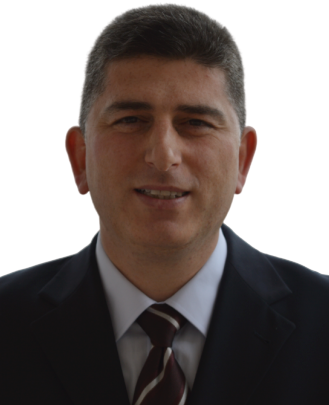
\includegraphics[width=1in,height=1.25in,clip,keepaspectratio]{figures/foto_mustafa.jpg}}]{Mustafa Namdar}
    (Member, IEEE) received the B.Sc. and Ph.D. degrees in electronics and communications engineering from Yildiz Technical University, Istanbul, Turkiye. From 2000 to 2011, he was with Turkcell, Istanbul, Turkiye, where he participated in several wireless communications projects. He is currently an Associate Professor with the Department of Electrical and Electronics Engineering, Kutahya Dumlupinar University, Kutahya, Turkiye. His research interests include cognitive radio networks, interference alignment, nonorthogonal multiple access (NOMA), reconfigurable intelligent surfaces (RIS), and integrated sensing and communication (ISAC).
\end{IEEEbiography}

\end{document}

